\documentclass[11pt,fleqn, openany]{book} % Default font size and left-justified equations

%%%%%%%%%%%%%%%%%%%%%%%%%%%%%%%%%%%%%%%%%
% The Legrand Orange Book
% Structural Definitions File
% Version 2.1 (26/09/2018)
%
% Original author:
% Mathias Legrand (legrand.mathias@gmail.com) with modifications by:
% Vel (vel@latextemplates.com)
% 
% This file was downloaded from:
% http://www.LaTeXTemplates.com
%
% License:
% CC BY-NC-SA 3.0 (http://creativecommons.org/licenses/by-nc-sa/3.0/)
%
%%%%%%%%%%%%%%%%%%%%%%%%%%%%%%%%%%%%%%%%%

%----------------------------------------------------------------------------------------
%	VARIOUS REQUIRED PACKAGES AND CONFIGURATIONS
%----------------------------------------------------------------------------------------

\usepackage[table]{xcolor}

\usepackage{graphicx}
\usepackage{tabularx} % Required for including pictures
\usepackage{pgf,tikz,tkz-tab,eurosym,yhmath, stmaryrd}
\usepackage{pgfplots}
\usepackage{mathrsfs}
\usetikzlibrary{patterns}
\usetikzlibrary{trees}
\graphicspath{{../../Pictures/}}
\usepackage{multicol} 


\usepackage[english]{babel} % English language/hyphenation
\usepackage{icomma}
\usepackage{enumitem} % Customize lists
\setlist{nolistsep, nosep, nolistsep} % Reduce spacing between bullet points and numbered lists

\usepackage{booktabs} % Required for nicer horizontal rules in tables

 % Required for specifying colors by name


\definecolor{ocre}{RGB}{243,102,25} % Define the orange color used for highlighting throughout the book

\usepackage{listings}

\definecolor{codegreen}{rgb}{0,0.6,0}
\definecolor{codegray}{rgb}{0.5,0.5,0.5}
\definecolor{codepurple}{rgb}{0.58,0,0.82}
\definecolor{backcolour}{rgb}{0.95,0.95,0.92}

\lstdefinestyle{mystyle}{
    backgroundcolor=\color{backcolour},   
    commentstyle=\color{codegreen},
    keywordstyle=\color{magenta},
    numberstyle=\tiny\color{codegray},
    stringstyle=\color{codepurple},
    basicstyle=\ttfamily\footnotesize,
    breakatwhitespace=false,         
    breaklines=true,                 
    captionpos=b,                    
    keepspaces=true,                 
    numbers=left,                    
    numbersep=5pt,                  
    showspaces=false,                
    showstringspaces=false,
    showtabs=false,                  
    tabsize=2
}

\lstset{style=mystyle}

%----------------------------------------------------------------------------------------
% Paramétrage XSIM
%----------------------------------------------------------------------------------------

\usepackage[no-files]{xsim}


\DeclareExerciseEnvironmentTemplate{myex}{%
    \textbf{%
      \hypertarget{ex:\ExerciseID}{\sffamily{\ensuremath{\blacktriangleright}} Exercice \GetExerciseProperty{counter} \GetExerciseProperty{subtitle} --}
      \hyperlink{sol:\ExerciseID}{Voir le corrigé}%
    }\par
}{\par\smallskip}

\DeclareExerciseEnvironmentTemplate{mysol}{%
    \textbf{%
      \hypertarget{sol:\ExerciseID}{\sffamily{\ensuremath{\blacktriangleright}} Correction \GetExerciseProperty{counter} --}
      \hyperlink{ex:\ExerciseID}{Voir l'énoncé}%
    }\par
}{\par\medskip}

\xsimsetup{
  exercise/template = myex ,
  solution/template = mysol 
}

%Collection exercices

\DeclareExerciseTagging{topic}

\xsimsetup{collect}

%----------------------------------------------------------------------------------------
% SYMBOLES
%----------------------------------------------------------------------------------------

\newcommand\imCMsym[4][\mathord]{%
  \DeclareFontFamily{U} {#2}{}
  \DeclareFontShape{U}{#2}{m}{n}{
    <-6> #25
    <6-7> #26
    <7-8> #27
    <8-9> #28
    <9-10> #29
    <10-12> #210
    <12-> #212}{}
  \DeclareSymbolFont{CM#2} {U} {#2}{m}{n}
  \DeclareMathSymbol{#4}{#1}{CM#2}{#3}
}
\newcommand\alsoimCMsym[4][\mathord]{\DeclareMathSymbol{#4}{#1}{CM#2}{#3}}

\imCMsym{cmmi}{124}{\CMjmath}

\newcommand{\Oij}{(O\,;\,\vec{\imath}\,,\, \vec{\CMjmath} )}
\newcommand{\Oijk}{(O\,;\,\vec{\imath}\,,\, \vec{\CMjmath}\,,\,\vec{k})}

\newcommand\e{\mathrm{e}}
\newcommand\R{\mathbb{R}}
\newcommand\N{\mathbb{N}}


%----------------------------------------------------------------------------------------
%	MARGINS
%----------------------------------------------------------------------------------------

\usepackage{geometry} % Required for adjusting page dimensions and margins

\geometry{
	paper=a4paper, % Paper size, change to letterpaper for US letter size
	top=3cm, % Top margin
	bottom=3cm, % Bottom margin
	left=2cm, % Left margin
	right=2cm, % Right margin
	headheight=14pt, % Header height
	footskip=1.4cm, % Space from the bottom margin to the baseline of the footer
	headsep=10pt, % Space from the top margin to the baseline of the header
	%showframe, % Uncomment to show how the type block is set on the page
}

\setlength{\parindent}{0pt}
\parskip=5pt



%----------------------------------------------------------------------------------------
%	FONTS
%----------------------------------------------------------------------------------------

\usepackage{avant} % Use the Avantgarde font for headings
\usepackage{times} % Use the Times font for headings
\usepackage{mathptmx} % Use the Adobe Times Roman as the default text font together with math symbols from the Sym­bol, Chancery and Com­puter Modern fonts

%\usepackage{microtype} % Slightly tweak font spacing for aesthetics
%\usepackage[utf8]{inputenc} % Required for including letters with accents
\usepackage[T1]{fontenc} % Use 8-bit encoding that has 256 glyphs

%----------------------------------------------------------------------------------------
%	BIBLIOGRAPHY AND INDEX
%----------------------------------------------------------------------------------------

\usepackage[style=numeric,citestyle=numeric,sorting=nyt,sortcites=true,autopunct=true,babel=hyphen,hyperref=true,abbreviate=false,backref=true,backend=biber]{biblatex}
\addbibresource{bibliography.bib} % BibTeX bibliography file
\defbibheading{bibempty}{}

\usepackage{calc} % For simpler calculation - used for spacing the index letter headings correctly
\usepackage{makeidx} % Required to make an index
\makeindex % Tells LaTeX to create the files required for indexing

%----------------------------------------------------------------------------------------
%	MAIN TABLE OF CONTENTS
%----------------------------------------------------------------------------------------

\usepackage{titletoc} % Required for manipulating the table of contents

\contentsmargin{0cm} % Removes the default margin

% Part text styling (this is mostly taken care of in the PART HEADINGS section of this file)
\titlecontents{part}
	[0cm] % Left indentation
	{\addvspace{20pt}\bfseries} % Spacing and font options for parts
	{}
	{}
	{}

% Chapter text styling
\titlecontents{chapter}
	[1.25cm] % Left indentation
	{\addvspace{12pt}\large\sffamily\bfseries} % Spacing and font options for chapters
	{\color{ocre!60}\contentslabel[\Large\thecontentslabel]{1.25cm}\color{ocre}} % Formatting of numbered sections of this type
	{\color{ocre}} % Formatting of numberless sections of this type
	{\color{ocre!60}\normalsize\;\titlerule*[.5pc]{.}\;\thecontentspage} % Formatting of the filler to the right of the heading and the page number

% Section text styling
\titlecontents{section}
	[1.25cm] % Left indentation
	{\addvspace{3pt}\sffamily\bfseries} % Spacing and font options for sections
	{\contentslabel[\thecontentslabel]{1.25cm}} % Formatting of numbered sections of this type
	{} % Formatting of numberless sections of this type
	{\hfill\color{black}\thecontentspage} % Formatting of the filler to the right of the heading and the page number

% Subsection text styling
\titlecontents{subsection}
	[1.25cm] % Left indentation
	{\addvspace{1pt}\sffamily\small} % Spacing and font options for subsections
	{\contentslabel[\thecontentslabel]{1.25cm}} % Formatting of numbered sections of this type
	{} % Formatting of numberless sections of this type
	{\ \titlerule*[.5pc]{.}\;\thecontentspage} % Formatting of the filler to the right of the heading and the page number

% Figure text styling
\titlecontents{figure}
	[1.25cm] % Left indentation
	{\addvspace{1pt}\sffamily\small} % Spacing and font options for figures
	{\thecontentslabel\hspace*{1em}} % Formatting of numbered sections of this type
	{} % Formatting of numberless sections of this type
	{\ \titlerule*[.5pc]{.}\;\thecontentspage} % Formatting of the filler to the right of the heading and the page number

% Table text styling
\titlecontents{table}
	[1.25cm] % Left indentation
	{\addvspace{1pt}\sffamily\small} % Spacing and font options for tables
	{\thecontentslabel\hspace*{1em}} % Formatting of numbered sections of this type
	{} % Formatting of numberless sections of this type
	{\ \titlerule*[.5pc]{.}\;\thecontentspage} % Formatting of the filler to the right of the heading and the page number

%----------------------------------------------------------------------------------------
%	MINI TABLE OF CONTENTS IN PART HEADS
%----------------------------------------------------------------------------------------

% Chapter text styling
\titlecontents{lchapter}
	[0em] % Left indentation
	{\addvspace{15pt}\large\sffamily\bfseries} % Spacing and font options for chapters
	{\color{ocre}\contentslabel[\Large\thecontentslabel]{1.25cm}\color{ocre}} % Chapter number
	{}  
	{\color{ocre}\normalsize\sffamily\bfseries\;\titlerule*[.5pc]{.}\;\thecontentspage} % Page number

% Section text styling
\titlecontents{lsection}
	[0em] % Left indentation
	{\sffamily\small} % Spacing and font options for sections
	{\contentslabel[\thecontentslabel]{1.25cm}} % Section number
	{}
	{}

% Subsection text styling (note these aren't shown by default, display them by searchings this file for tocdepth and reading the commented text)
\titlecontents{lsubsection}
	[.5em] % Left indentation
	{\sffamily\footnotesize} % Spacing and font options for subsections
	{\contentslabel[\thecontentslabel]{1.25cm}}
	{}
	{}

%----------------------------------------------------------------------------------------
%	HEADERS AND FOOTERS
%----------------------------------------------------------------------------------------


\usepackage{fancyhdr} % Required for header and footer configuration

\pagestyle{fancy}
\renewcommand{\chaptermark}[1]{\markboth{\sffamily\normalsize\bfseries\ \thechapter.\ #1}{}} % Chapter text font settings
\renewcommand{\sectionmark}[1]{\markright{\sffamily\normalsize\thesection\hspace{5pt}#1}{}} % Section text font settings
\fancyhf{} \fancyhead[LE,RO]{\sffamily\normalsize\thepage} % Font setting for the page number in the header
\fancyhead[LO]{\rightmark} % Print the nearest section name on the left side of odd pages
\fancyhead[RE]{\leftmark} % Print the current chapter name on the right side of even pages

\fancyfoot[L]{Jason LAPEYRONNIE}
\fancyfoot[R]{\href{http://mathoutils.fr}{http://mathoutils.fr}} % Uncomment to include a footer

\renewcommand{\headrulewidth}{0.5pt} % Thickness of the rule under the header
\renewcommand{\footrulewidth}{0.5pt} % Thickness of the rule under the header

\fancypagestyle{plain}{% Style for when a plain pagestyle is specified
	\fancyhead{}\renewcommand{\headrulewidth}{0pt}%
}

% Removes the header from odd empty pages at the end of chapters
\makeatletter
\renewcommand{\cleardoublepage}{
\clearpage\ifodd\c@page\else
\hbox{}
\vspace*{\fill}
\thispagestyle{empty}
\newpage
\fi}

%----------------------------------------------------------------------------------------
%	THEOREM STYLES
%----------------------------------------------------------------------------------------

\usepackage{amsmath,amsfonts,amssymb,amsthm} % For math equations, theorems, symbols, etc

\newcommand{\intoo}[2]{\mathopen{]}#1\,;#2\mathclose{[}}
\newcommand{\ud}{\mathop{\mathrm{{}d}}\mathopen{}}
\newcommand{\intff}[2]{\mathopen{[}#1\,;#2\mathclose{]}}
\renewcommand{\qedsymbol}{$\blacksquare$}
\newtheorem{notation}{Notation}[section]

% Boxed/framed environments
\newtheoremstyle{ocrenumbox}% Theorem style name
{0pt}% Space above
{0pt}% Space below
{\normalfont}% Body font
{}% Indent amount
{\small\bf\sffamily\color{ocre}}% Theorem head font
{\;:\;}% Punctuation after theorem head
{0.25em}% Space after theorem head
{\small\sffamily\color{ocre}\thmname{#1}\nobreakspace\thmnumber{\@ifnotempty{#1}{}\@upn{#2}}% Theorem text (e.g. Theorem 2.1)
\thmnote{\nobreakspace\the\thm@notefont\sffamily\bfseries\color{black}---\nobreakspace#3}} % Optional theorem note

\newtheoremstyle{blacknumex}% Theorem style name
{5pt}% Space above
{10pt}% Space below
{\normalfont}% Body font
{} % Indent amount
{\small\bf\sffamily}% Theorem head font
{\;:\;}% Punctuation after theorem head
{0.25em}% Space after theorem head
{\small\sffamily{\tiny\ensuremath{\blacksquare}}\nobreakspace\thmname{#1}\nobreakspace\thmnumber{\@ifnotempty{#1}{}\@upn{#2}}% Theorem text (e.g. Theorem 2.1)
\thmnote{\nobreakspace\the\thm@notefont\sffamily\bfseries---\nobreakspace#3}}% Optional theorem note

\newtheoremstyle{blacknumexo}% Theorem style name
{15pt}% Space above
{10pt}% Space below
{\normalfont}% Body font
{} % Indent amount
{\small\bf\sffamily}% Theorem head font
{}% Punctuation after theorem head
{0.5em}% Space after theorem head
{\small\sffamily{\ensuremath{\blacktriangleright}}\nobreakspace\thmname{#1}\nobreakspace\thmnumber{\@ifnotempty{#1}{}\@upn{#2}}% Theorem text (e.g. Theorem 2.1)
\thmnote{\nobreakspace\the\thm@notefont\sffamily\bfseries---\nobreakspace#3} \\}% Optional theorem note



\newtheoremstyle{blacknumbox} % Theorem style name
{0pt}% Space above
{5pt}% Space below
{}% Body font
{}% Indent amount
{\large\bf\sffamily}% Theorem head font
{\;:\;}% Punctuation after theorem head
{0.25em}% Space after theorem head
{\small\sffamily\thmname{#1}\nobreakspace\thmnumber{\@ifnotempty{#1}{}\@upn{#2}}% Theorem text (e.g. Theorem 2.1)
\thmnote{\nobreakspace\the\thm@notefont\sffamily\bfseries---\nobreakspace#3}}% Optional theorem note

% Non-boxed/non-framed environments
\newtheoremstyle{ocrenum}% Theorem style name
{5pt}% Space above
{5pt}% Space below
{\normalfont}% Body font
{}% Indent amount
{\small\bf\sffamily\color{ocre}}% Theorem head font
{\;:\;}% Punctuation after theorem head
{0.25em}% Space after theorem head
{\small\sffamily\color{ocre}\thmname{#1}\nobreakspace\thmnumber{\@ifnotempty{#1}{}\@upn{#2}}% Theorem text (e.g. Theorem 2.1)
\thmnote{\nobreakspace\the\thm@notefont\sffamily\bfseries\color{black}---\nobreakspace#3}} % Optional theorem note
\makeatother

% Defines the theorem text style for each type of theorem to one of the three styles above
\newcounter{dummy} 
\newcounter{thm}
\newcounter{correction}
\newcounter{qst}
\theoremstyle{ocrenumbox}
\newtheorem{theoremeT}[dummy]{Théorème}
\newtheorem{exerciseT}{Propriété}
\newtheorem{principeT}{Principe}
\theoremstyle{blacknumex}
\newtheorem{exampleT}{Exemple}
\theoremstyle{blacknumexo}
\newtheorem{exo}[thm]{Exercice}
\newtheorem{corr}[correction]{Correction}
\newtheorem{quest}[qst]{Question}
\theoremstyle{blacknumbox}
\newtheorem{vocabulary}{Vocabulary}[section]
\newtheorem{definitionT}{Définition}
\newtheorem{corollaryT}[dummy]{Corollary}
\theoremstyle{ocrenum}
\newtheorem{proofT}[dummy]{Démonstration}


%----------------------------------------------------------------------------------------
%	DEFINITION OF COLORED BOXES
%----------------------------------------------------------------------------------------

\RequirePackage[framemethod=default]{mdframed} % Required for creating the theorem, definition, exercise and corollary boxes

% Theorem box
\newmdenv[skipabove=7pt,
skipbelow=7pt,
backgroundcolor=black!5,
linecolor=ocre,
innerleftmargin=5pt,
innerrightmargin=5pt,
innertopmargin=10pt,
leftmargin=0cm,
rightmargin=0cm,
innerbottommargin=5pt]{tBox}

%Proposition box	  
\newmdenv[skipabove=7pt,
skipbelow=7pt,
rightline=false,
leftline=true,
topline=false,
bottomline=false,
backgroundcolor=ocre!10,
linecolor=ocre,
innerleftmargin=5pt,
innerrightmargin=5pt,
innertopmargin=10pt,
innerbottommargin=3pt,
leftmargin=0cm,
rightmargin=0cm,
linewidth=4pt]{eBox}	

% Definition box
\newmdenv[skipabove=7pt,
backgroundcolor=ocre!4,
skipbelow=7pt,
rightline=false,
leftline=true,
topline=false,
bottomline=false,
linecolor=ocre,
innerleftmargin=5pt,
innerrightmargin=5pt,
innertopmargin=10pt,
leftmargin=0cm,
rightmargin=0cm,
linewidth=4pt,
innerbottommargin=5pt]{dBox}	

% Corollary box
\newmdenv[skipabove=7pt,
skipbelow=7pt,
rightline=false,
leftline=true,
topline=false,
bottomline=false,
linecolor=gray,
backgroundcolor=black!5,
innerleftmargin=5pt,
innerrightmargin=5pt,
innertopmargin=5pt,
leftmargin=0cm,
rightmargin=0cm,
linewidth=4pt,
innerbottommargin=5pt]{cBox}

\newmdenv[skipabove=7pt,
skipbelow=7pt,
backgroundcolor=black!5,
innerleftmargin=5pt,
topline=false,
bottomline=false,
rightline=false,
leftline=false,
innerrightmargin=5pt,
innertopmargin=5pt,
leftmargin=0cm,
rightmargin=0cm,
innerbottommargin=5pt]{xBox}

% Creates an environment for each type of theorem and assigns it a theorem text style from the "Theorem Styles" section above and a colored box from above
\newenvironment{theorem}{\begin{tBox}\begin{theoremeT}}{\end{theoremeT}\end{tBox}}

\newenvironment{exo2}{\noindent \begin{exo}\item\relax \noindent \begin{eBox}\item\relax}{\end{eBox}\end{exo}}


\newenvironment{proposition}{\begin{eBox}\begin{exerciseT}}{\hfill{\color{ocre}}\end{exerciseT}\end{eBox}}		

\newenvironment{principe}{\begin{eBox}\begin{principeT}}{\hfill{\color{ocre}}\end{principeT}\end{eBox}}	
		  
\newenvironment{definition}{\begin{dBox}\begin{definitionT}}{\end{definitionT}\end{dBox}}	

\newenvironment{example}{\begin{xBox}\begin{exampleT}}{\hfill{\tiny\ensuremath{\blacksquare}}\end{exampleT}\end{xBox}}

\newenvironment{demonstration}{\begin{proofT}}{\hfill{\tiny\ensuremath{\square}}\end{proofT}}		
\newenvironment{corollary}{\begin{cBox}\begin{corollaryT}}{\end{corollaryT}\end{cBox}}	

%----------------------------------------------------------------------------------------
%	REMARK ENVIRONMENT
%----------------------------------------------------------------------------------------

\newenvironment{remark}{\par\vspace{5pt}\small % Vertical white space above the remark and smaller font size
\begin{list}{}{
\leftmargin=25pt % Indentation on the left
\rightmargin=15pt}\item\ignorespaces % Indentation on the right
\makebox[-2.5pt]{
\begin{tikzpicture}[overlay]
\node[draw=ocre!60,line width=1pt,circle,fill=ocre!25,font=\sffamily\bfseries,inner sep=2pt,outer sep=0pt] at (-15pt,0pt){\textcolor{ocre}{R}};\end{tikzpicture}} % Orange R in a circle
\advance\baselineskip -1pt}{\end{list}\vskip5pt} % Tighter line spacing and white space after remark

%----------------------------------------------------------------------------------------
%	SECTION NUMBERING IN THE MARGIN
%----------------------------------------------------------------------------------------

\makeatletter
\renewcommand{\@seccntformat}[1]{\llap{\textcolor{ocre}{\csname the#1\endcsname}\hspace{1em}}}                    
\renewcommand{\section}{\@startsection{section}{1}{\z@}
{-4ex \@plus -1ex \@minus -.4ex}
{1ex \@plus.2ex }
{\normalfont\LARGE\sffamily\bfseries}}
\renewcommand{\subsection}{\@startsection {subsection}{2}{\z@}
{-3ex \@plus -0.1ex \@minus -.4ex}
{0.5ex \@plus.2ex }
{\normalfont\sffamily\bfseries}}
\renewcommand{\subsubsection}{\@startsection {subsubsection}{3}{\z@}
{-2ex \@plus -0.1ex \@minus -.2ex}
{.2ex \@plus.2ex }
{\normalfont\small\sffamily\bfseries}}                        
\renewcommand\paragraph{\@startsection{paragraph}{4}{\z@}
{-2ex \@plus-.2ex \@minus .2ex}
{.1ex}
{\normalfont\small\sffamily\bfseries}}

%----------------------------------------------------------------------------------------
%	PART HEADINGS
%----------------------------------------------------------------------------------------

% Numbered part in the table of contents
\newcommand{\@mypartnumtocformat}[2]{%
	\setlength\fboxsep{0pt}%
	\noindent\colorbox{ocre!20}{\strut\parbox[c][.7cm]{\ecart}{\color{ocre!70}\Large\sffamily\bfseries\centering#1}}\hskip\esp\colorbox{ocre!40}{\strut\parbox[c][.7cm]{\linewidth-\ecart-\esp}{\Large\sffamily\centering#2}}%
}

% Unnumbered part in the table of contents
\newcommand{\@myparttocformat}[1]{%
	\setlength\fboxsep{0pt}%
	\noindent\colorbox{ocre!40}{\strut\parbox[c][.7cm]{\linewidth}{\Large\sffamily\centering#1}}%
}

\newlength\esp
\setlength\esp{4pt}
\newlength\ecart
\setlength\ecart{1.2cm-\esp}
\newcommand{\thepartimage}{}%
\newcommand{\partimage}[1]{\renewcommand{\thepartimage}{#1}}%
\def\@part[#1]#2{%
\ifnum \c@secnumdepth >-2\relax%
\refstepcounter{part}%
\addcontentsline{toc}{part}{\texorpdfstring{\protect\@mypartnumtocformat{\thepart}{#1}}{\partname~\thepart\ ---\ #1}}
\else%
\addcontentsline{toc}{part}{\texorpdfstring{\protect\@myparttocformat{#1}}{#1}}%
\fi%
\startcontents%
\markboth{}{}%
{\thispagestyle{empty}%
\begin{tikzpicture}[remember picture,overlay]%
\node at (current page.north west){\begin{tikzpicture}[remember picture,overlay]%	
\fill[ocre!20](0cm,0cm) rectangle (\paperwidth,-\paperheight);
\node[anchor=north] at (4cm,-3.25cm){\color{ocre!40}\fontsize{220}{100}\sffamily\bfseries\thepart}; 
\node[anchor=south east] at (\paperwidth-1cm,-\paperheight+1cm){\parbox[t][][t]{8.5cm}{
\printcontents{l}{0}{\setcounter{tocdepth}{1}}% The depth to which the Part mini table of contents displays headings; 0 for chapters only, 1 for chapters and sections and 2 for chapters, sections and subsections
}};
\node[anchor=north east] at (\paperwidth-1.5cm,-3.25cm){\parbox[t][][t]{15cm}{\strut\raggedleft\color{white}\fontsize{30}{30}\sffamily\bfseries#2}};
\end{tikzpicture}};
\end{tikzpicture}}%
\@endpart}
\def\@spart#1{%
\startcontents%
\phantomsection
{\thispagestyle{empty}%
\begin{tikzpicture}[remember picture,overlay]%
\node at (current page.north west){\begin{tikzpicture}[remember picture,overlay]%	
\fill[ocre!20](0cm,0cm) rectangle (\paperwidth,-\paperheight);
\node[anchor=north east] at (\paperwidth-1.5cm,-3.25cm){\parbox[t][][t]{15cm}{\strut\raggedleft\color{white}\fontsize{30}{30}\sffamily\bfseries#1}};
\end{tikzpicture}};
\end{tikzpicture}}
\addcontentsline{toc}{part}{\texorpdfstring{%
\setlength\fboxsep{0pt}%
\noindent\protect\colorbox{ocre!40}{\strut\protect\parbox[c][.7cm]{\linewidth}{\Large\sffamily\protect\centering #1\quad\mbox{}}}}{#1}}%
\@endpart}
\def\@endpart{\vfil\newpage
\if@twoside
\if@openright
\null
\thispagestyle{empty}%
\newpage
\fi
\fi
\if@tempswa
\twocolumn
\fi}

%----------------------------------------------------------------------------------------
%	CHAPTER HEADINGS
%----------------------------------------------------------------------------------------

% A switch to conditionally include a picture, implemented by Christian Hupfer
\newif\ifusechapterimage
\usechapterimagetrue
\newcommand{\thechapterimage}{}%
\newcommand{\chapterimage}[1]{\ifusechapterimage\renewcommand{\thechapterimage}{#1}\fi}%
\newcommand{\autodot}{.}
\def\@makechapterhead#1{%
{\parindent \z@ \raggedright \normalfont
\ifnum \c@secnumdepth >\m@ne
\if@mainmatter
\begin{tikzpicture}[remember picture,overlay]
\node at (current page.north west)
{\begin{tikzpicture}[remember picture,overlay]
\node[anchor=north west,inner sep=0pt] at (0,0) {\ifusechapterimage\includegraphics[width=\paperwidth]{\thechapterimage}\fi};
\draw[anchor=west] (\Gm@lmargin,-3cm) node [line width=2pt,rounded corners=15pt,draw=ocre,fill=white,fill opacity=0.5,inner sep=15pt]{\strut\makebox[22cm]{}};
\draw[anchor=west] (\Gm@lmargin+.3cm,-3cm) node {\huge\sffamily\bfseries\color{black}\thechapter\autodot~#1\strut};
\end{tikzpicture}};
\end{tikzpicture}
\else
\begin{tikzpicture}[remember picture,overlay]
\node at (current page.north west)
{\begin{tikzpicture}[remember picture,overlay]
\node[anchor=north west,inner sep=0pt] at (0,0) {\ifusechapterimage\includegraphics[width=\paperwidth]{\thechapterimage}\fi};
\draw[anchor=west] (\Gm@lmargin,-3cm) node [line width=2pt,rounded corners=15pt,draw=ocre,fill=white,fill opacity=0.5,inner sep=15pt]{\strut\makebox[22cm]{}};
\draw[anchor=west] (\Gm@lmargin+.3cm,-3cm) node {\huge\sffamily\bfseries\color{black}#1\strut};
\end{tikzpicture}};
\end{tikzpicture}
\fi\fi\par\vspace*{50\p@}}}

%-------------------------------------------

\def\@makeschapterhead#1{%
\begin{tikzpicture}[remember picture,overlay]
\node at (current page.north west)
{\begin{tikzpicture}[remember picture,overlay]
\node[anchor=north west,inner sep=0pt] at (0,0) {\ifusechapterimage\includegraphics[width=\paperwidth]{\thechapterimage}\fi};
\draw[anchor=west] (\Gm@lmargin,-3cm) node [line width=2pt,rounded corners=15pt,draw=ocre,fill=white,fill opacity=0.5,inner sep=15pt]{\strut\makebox[22cm]{}};
\draw[anchor=west] (\Gm@lmargin+.3cm,-3cm) node {\huge\sffamily\bfseries\color{black}#1\strut};
\end{tikzpicture}};
\end{tikzpicture}
\par\vspace*{50\p@}}
\makeatother

%----------------------------------------------------------------------------------------
%	LINKS
%----------------------------------------------------------------------------------------

\usepackage{hyperref}
\hypersetup{hidelinks,backref=true,pagebackref=true,hyperindex=true,colorlinks=false,breaklinks=true,urlcolor=ocre,bookmarks=true,bookmarksopen=false}

\usepackage{bookmark}
\bookmarksetup{
open,
numbered,
addtohook={%
\ifnum\bookmarkget{level}=0 % chapter
\bookmarksetup{bold}%
\fi
\ifnum\bookmarkget{level}=-1 % part
\bookmarksetup{color=ocre,bold}%
\fi
}
}

\renewcommand*\thesection{\arabic{section}}

\newcommand*{\coord}[3]{% 
  \ensuremath{\overrightarrow{#1}\, 
    \begin{pmatrix} 
      #2\\ 
      #3 
    \end{pmatrix}}}
    
  \newcommand*{\coordb}[2]{% 
  \ensuremath{ 
    \begin{pmatrix} 
      #1\\ 
      #2 
    \end{pmatrix}}}

\newcommand*{\coorde}[4]{% 
  \renewcommand{\arraystretch}{1}\ensuremath{\overrightarrow{#1}\, 
    \begin{pmatrix} 
      #2\\ 
      #3 \\
      #4
    \end{pmatrix}}}    
  \newcommand*{\coordbe}[3]{% 
 \renewcommand{\arraystretch}{1} \ensuremath{ 
    \begin{pmatrix} 
      #1\\ 
      #2 \\
      #3
    \end{pmatrix}}}  
    
\newcommand{\Card}{\mathrm{Card}}



\begin{document}

\chapterimage{../../Pictures/background}



\chapter{Cours : Continuité}



\section{Continuité d'une fonction réelle}

\begin{definition}[Continuité] Soit $f$ une fonction définie sur un intervalle $I$. Soit $a\in I$.
\begin{itemize}
\item On dit que $f$ est \textit{continue} en $a$ si $f$ admet une limite en $a$, par valeurs supérieures et par valeurs inférieures, et que  $\displaystyle \lim_{x \to a} f(x)=\displaystyle \lim_{x \to a^+} f(x)=\displaystyle \lim_{x \to a^-} f(x)=f(a)$.
\item On dit que $f$ est \textit{continue} sur $I$ si $f$ est continue en tout réel de $I$.
\end{itemize}\end{definition}

\begin{example} Jusqu'ici, les fonction de référence rencontrées étaient continues sur leur domaine de définition : fonctions polynômes ou quotients de polynômes, exponentielle, racine carrée, sinus, cosinus, valeur absolue...\end{example}


\begin{example}On considère la fonction $f$ dont la courbe représentative $\mathcal{C}_f$ est donnée ci-dessous.


\begin{minipage}{0.5\linewidth}\begin{center}

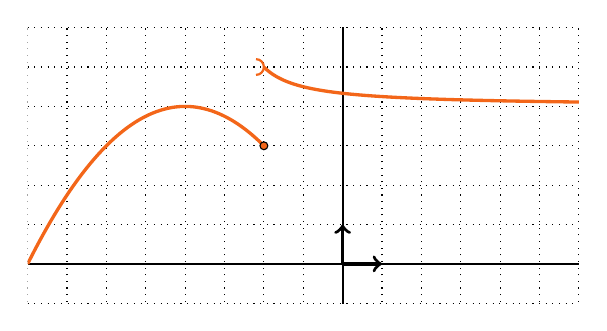
\begin{tikzpicture}[scale=0.5]
\clip (-8,-1) rectangle (6,6);
\draw [thick] (-8,0)--(22,0);
\draw [thick] (0,-4)--(0,28);
\draw [->, very thick] (0,0)--(1,0);
\draw [->,very thick] (0,0)--(0,1);
\draw [ thin, dotted] (-8,-4) grid (22,28);

\draw [very thick, ocre, domain = -2:6, samples =200] plot (\x,{4+1/(\x+3)}) ;
\draw [very thick, ocre, domain = -8:-2, samples =200] plot (\x,{-0.25*\x*\x-2*\x}) ;

\draw [fill=ocre] (-2,3) circle(0.1) ;
\draw [ocre, thick] (-2.2,4.8) arc (-90:90:0.2) ;

\end{tikzpicture}

\end{center}\end{minipage}\hfill\begin{minipage}{0.45\linewidth}


On remarque que 
\begin{itemize}
\item $\displaystyle \lim_{x \to (-2)^-}f(x)=$ 
\item $\displaystyle \lim_{x \to (-2)^+}f(x)=$\end{itemize}
 Ces deux valeurs sont différentes, la fonction $f$ n'est pas continue en 2. 
 
 Graphiquement, on voit que la courbe de la fonction fait un "saut" en $x=-2$.\end{minipage}\end{example}

\begin{example} On considère la fonction \renewcommand{\arraystretch}{1.2}$f:x\mapsto \left\{ \begin{array}{ll}
2x+9 & \text{si }x<-2\\
x^2+1 & \text{si }-2\leqslant x < 3\\
4x-4 & \text{si } x \geqslant 3
\end{array}\right.$ définie sur $\mathbb{R}$.

\begin{minipage}{0.7\linewidth}
La fonction $f$ est continue sur $]-\infty;-2[$, $]-2;3[$ et $]3;+\infty[$. 

Il faut étudier la continuité aux bords de chaque intervalle.

\paragraph{Continuité en $-2$}

\vskip80pt

\paragraph{Continuité en $3$}
\vskip80pt

\end{minipage}\hfill\begin{minipage}{0.25\linewidth}


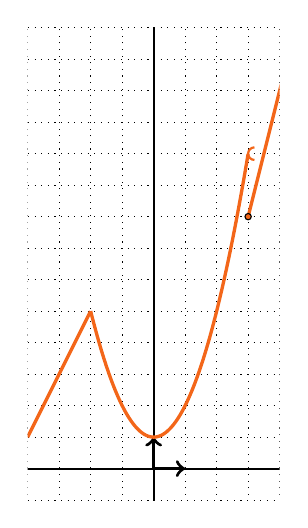
\begin{tikzpicture}[scale=0.4]
\clip (-4,-1) rectangle (4,14);
\draw [thick] (-8,0)--(22,0);
\draw [thick] (0,-4)--(0,28);
\draw [->, very thick] (0,0)--(1,0);
\draw [->,very thick] (0,0)--(0,1);
\draw [ thin, dotted] (-8,-4) grid (22,28);

\draw [very thick, ocre, domain = -4:-2, samples =200] plot (\x,{2*\x+9}) ;
\draw [very thick, ocre, domain = -2:3, samples =200] plot (\x,{\x*\x+1}) ;
\draw [very thick, ocre, domain = 3:6, samples =200] plot (\x,{4*\x-4}) ;

\draw [fill=ocre] (3,8) circle(0.1) ;
\draw [ocre, thick] (3.2,10.2) arc (90:270:0.2) ;

\end{tikzpicture}

\end{minipage}
\vskip50pt

\end{example}

\newpage

\begin{proposition} La somme et le produit de fonctions continues sur un intervalle $I$ sont continus sur $I$.\end{proposition}

\begin{example} La fonction $x\mapsto \cos(x)(x^2+3\sqrt{x})-\sin(x)e^x$ est continue sur $\mathbb{R}_+$.\end{example}

\begin{theorem} Soit $f$ une fonction définie sur un intervalle $I$. 

Si $f$ est dérivable sur $I$, alors $f$ est également continue sur $I$.\end{theorem}

La réciproque est fausse. La fonction $x\mapsto |x|$ est continue sur $\mathbb{R}$ mais n'est pas dérivable en 0.

\begin{minipage}{0.6\linewidth}
Il existe par ailleurs des fonctions continues sur $\mathbb{R}$ qui ne sont dérivables nulle part ! 

Les exemples les plus connus sont sans doute les fonctions de Weierstrass. Ce sont des courbes fractales : peu importe le niveau de zoom que l'on peut avoir sur la courbe, on verra toujours de nouveaux détails apparaître.
\end{minipage}\hfill \begin{minipage}{0.35\linewidth}
\begin{center}
\includegraphics[scale=0.15]{weierstrass}
\end{center}
\end{minipage}



\section{Suites et fonction continue}

\begin{proposition}[Image d'une suite convergente] Soit $I$ un intervalle et $(u_n)$ une suite telle que pour tout entier naturel $n$, $u_n \in I$. Soit $g$ une fonction définie sur l'intervalle $I$. 

Si la suite $(u_n)$ est convergente avec $\displaystyle\lim_{n\to +\infty} u_n=\ell \in I$ et si $g$ est \textbf{continue} en $\ell$, alors $\displaystyle\lim_{n\to +\infty} g(u_n)=g(\ell)$

En d'autres termes, $\displaystyle\lim_{n\to +\infty}g(u_n)=g(\displaystyle\lim_{n\to +\infty} u_n)$.\end{proposition}

\begin{example} Pour tout entier naturel non nul $n$, on note $u_n=\sqrt{9+\dfrac{1}{n}}$.

\vskip50pt

\end{example}

L'hypothèse de continuité est primordiale !
Pour tout réel $x$, notons $\lfloor x \rfloor$ la partie entière du réel $x$, c'est-à-dire le plus grand entier qui soit plus petit que $x$. Par exemple, $\lfloor 1,3 \rfloor = 1$.

Pour tout entier naturel non nul $n$, on note $u_n=1-\dfrac{1}{10^n}$. On a ainsi $u_0=0$, $u_1=0,9$, $u_2=0,999$, $u_3=0,9999$ etc.

\begin{itemize}
\item Pour tout entier naturel non nul, $\lfloor u_n \rfloor = 0$. On a alors $\displaystyle\lim_{n\to +\infty} \lfloor u_n \rfloor = 0$ ;
\item La suite $(u_n)$ est convergente et on a $\displaystyle\lim_{n\to +\infty} u_n = 1$. Ainsi, $\lfloor \displaystyle\lim_{n\to +\infty} u_n \rfloor=\lfloor 1 \rfloor=1$ ;
\item On a donc  $\displaystyle\lim_{n\to +\infty} \lfloor u_n \rfloor \neq \lfloor \displaystyle\lim_{n\to +\infty} u_n \rfloor$. 

On montre en fait que la fonction $x\mapsto  \lfloor x \rfloor$ n'est pas continue en 1.
\end{itemize}

\newpage

\begin{theorem}[Théorème du point fixe]Soit $I$ un intervalle, $g$ une fonction définie et continue sur $I$ et $(u_n)$ une suite telle que pour tout entier naturel $n$, $u_n \in I$ et $u_{n+1}=g(u_n)$.

On suppose que la suite $(u_n)$ est convergente, de limite $\ell\in I$. Alors $g(\ell)=\ell$.\end{theorem}

\begin{demonstration} Pour tout entier naturel $n$, on a $u_{n+1}=g(u_n)$.

\vskip50pt

\end{demonstration}

\begin{example}On définit la suite $(u_n)$ par $u_0=2$ et, pour tout entier $n$, $u_{n+1}=\sqrt{3u_n+4}$.

Montrons que la suite $(u_n)$ est croissante et que pour tout entier naturel $n$, $2 \leqslant u_n \leqslant 4$.

\vskip320pt


\end{example}

\newpage
\section{Théorème des valeurs intermédiaires}

\subsection{Cas général}

\begin{theorem}[Théorème des valeurs intermédiaires] Soit $f$ une fonction \textbf{continue} sur un intervalle $[a;b]$ et $k$ un réel compris entre $f(a)$ et $f(b)$.

Alors \textbf{il existe} (au moins) un réel $c$ dans $[a;b]$ tel que $f(c)=k$.\end{theorem}

\textbf{Illustration :} On représente une fonction $f$ ci-dessous.
\begin{center}

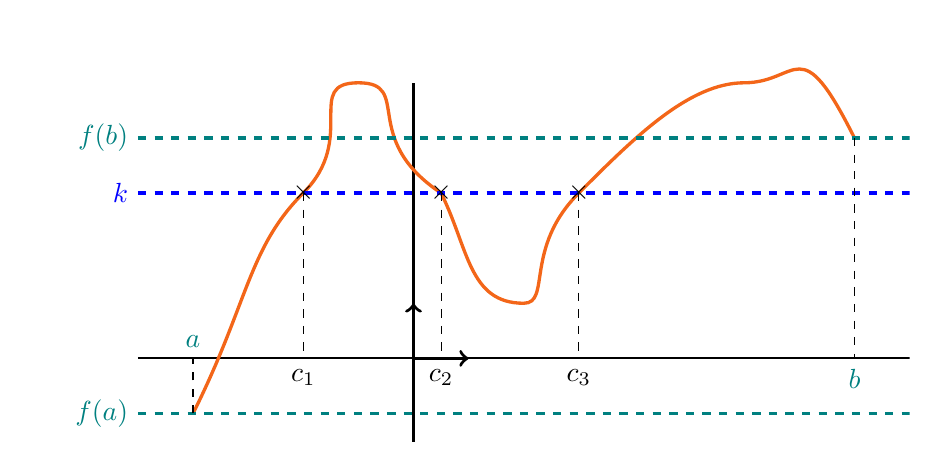
\begin{tikzpicture}[scale=0.7]
\clip (-7,-1.5) rectangle (9,6);
\draw [thick] (-5,0)--(9,0);
\draw [thick] (0,-3)--(0,5);
\draw [->, very thick] (0,0)--(1,0);
\draw [->,very thick] (0,0)--(0,1);

\draw [ocre, very thick] (-4,-1) .. controls (-3,1) and (-3,2) .. (-2,3)
.. controls (-1,4) and (-2,5) .. (-1,5) .. controls (0,5) and (-1,4) ..
(0.5,3) .. controls (1,2) and (1,1) .. (2,1) .. controls (2.5,1) and (2,2) ..
(3,3) .. controls (4,4) and (5,5) .. (6,5) .. controls (7,5) and (7,6) .. (8,4);

\draw [very thick,blue, dashed, domain = -5:9] plot (\x,3);
\draw [very thick,teal, dashed, domain = -5:9] plot (\x,4);
\draw [very thick,teal, dashed, domain = -5:9] plot (\x,-1);

\draw [teal] (-5,4) node[left] {$f(b)$};
\draw [teal] (-5,-1) node[left] {$f(a)$};
\draw [blue] (-5,3) node[left] {$k$};

\draw [very thick] (-2,3) node {$\times$};
\draw [very thick] (0.5,3) node {$\times$};
\draw [very thick] (3,3) node {$\times$};

\draw [dashed] (0.5,3) -- (0.5,0);
\draw [dashed] (-2,3) -- (-2,0);
\draw [dashed] (3,3) -- (3,0);

\draw [dashed] (-4,-1) -- (-4,0);
\draw [dashed] (8,4) -- (8,0);


\draw [very thick] (-2,0) node[below] {$c_1$};
\draw [very thick] (0.5,0) node[below] {$c_2$};
\draw [very thick] (3,0) node[below] {$c_3$};
\draw [teal, very thick] (8,0) node[below] {$b$};
\draw [teal, very thick] (-4,0) node[above] {$a$};

\end{tikzpicture}
\end{center}

Pour tout réel $k$ compris entre $f(a)$ et $f(b)$, $k$ possède au moins un antécédent par $f$. Dans cet exemple, il y en a trois. Le nom de ce théorème se justifie ainsi : une fonction continue qui passe d'une valeur $f(a)$ à une valeur $f(b)$ passe forcément au moins une fois par toutes les valeurs intermédiaires.




\begin{example} On considère la fonction $f:x\mapsto x^3-3x-1$, définie sur $\mathbb{R}$. La fonction $f$ est une fonction polynômiale, elle est donc continue. De plus, $f(-2)=-1$ et $f(2) = 3$.

Or, $0\in[-1;3]$. Ainsi, d'après le théorème des valeurs intermédiaires, il existe (au moins) un réel $c \in[-2;2]$ tel que $f(c)=0$.
\end{example}

Ce théorème ne nous donne aucune indication sur le nombre de ces solutions (en réalité, il y en a 3 sur cet intervalle). Nous verrons dans très peu de temps comment pallier ce problème.

Il est également possible d'utiliser les limites dans le théorème des valeurs intermédiaires.

\begin{theorem}[Théorème des valeurs intermédiaires] Soit $f$ une fonction \textbf{continue} sur un intervalle $]a;b[$ telle que $\displaystyle\lim_{x \to a^+}$ et $\displaystyle\lim_{x\to b^-}f(x)$ existent. Soit $k$ un réel strictement compris entre ces deux limites.

Alors \textbf{il existe} (au moins) un réel $c$ dans $]a;b[$ tel que $f(c)=k$.\end{theorem}


\begin{example}Soit $a$, $b$, $c$ et $d$ quatre réels avec $a> 0$. On considère la fonction $f:x\mapsto ax^3+bx^2+cx+d$, définie sur $\mathbb{R}$.

Pour tout réel non nul, $f(x)=x^3\left(a+\dfrac{b}{x}+\dfrac{c}{x^2}+\dfrac{d}{x^3}\right)$. Or, $\displaystyle\lim_{x\to +\infty}\left(a+\dfrac{b}{x}+\dfrac{c}{x^2}+\dfrac{d}{x^3}\right)=a>0$ et $\displaystyle\lim_{x\to+\infty}x^3=+\infty$. Ainsi, par produit, $\displaystyle\lim_{x\to+\infty}f(x)=+\infty$. De même, on montrer que $\displaystyle\lim_{x\to -\infty}f(x)=-\infty$.

Or, $0\in ]-\infty;+\infty[$. D'après le théorème des valeurs intermédiaires, il existe un réel $x$ tel que $f(x)=0$. Le même raisonnement vaut pour $a<0$ : nous venons de démontrer que tout polynôme de degré 3 admet au moins une racine réelle.\end{example}

\subsection{Fonctions strictement monotones}

\begin{theorem} Soit $f$ une fonction \textbf{continue} et \textbf{strictement monotone} sur un intervalle $[a;b]$ . Soit $k$ un réel strictement compris entre $f(a)$ et $f(b)$ (ou les limites en $a$ et $b$ de $f$). Alors il existe un \textbf{unique} réel $c \in ]a;b[$ tel que $f(c)=k$.\end{theorem}

Là encore, il est possible d'utiliser les limites de $f$ en $a$ et en $b$ si elles existent.

\begin{example} On considère la fonction $f:x\mapsto \dfrac{e^{x-1}}{x}$, définie sur $I=]0;+\infty[$.
Montrons que l'équation $f(x)=2$ possède exactement deux solutions sur l'intervalle $]0;+\infty[$.


\vskip450pt
   


 \end{example}

\newpage

\subsection{Algorithme de dichotomie}

Le théorème des valeurs intermédiaires nous assure de l'existence de solutions à une certaine équation. En revanche, il ne nous indique en rien la valeur de cette solution. Plusieurs algorithmes nous permettent néanmoins d'obtenir au moins une valeur approchée d'une solution de l'équation qui nous intéresse.

Considérons une fonction $f$ continue sur un intervalle $[a;b]$ et $k$ un réel compris entre $f(a)$ et $f(b)$. Dans cet exemple, on supposera par exemple que $f(a) \leqslant k \leqslant f(b)$. Le théorème des valeurs intermédiaires nous assure de l'existence d'un réel $c$ dans l'intervalle $[a;b]$ tel que $f(c)=k$. L'idée, pour obtenir une valeur approchée d'un tel réel, est d'évaluer la valeur prise par la fonction au milieu de l'intervalle $[a;b]$
\begin{itemize}
\item Si $f\left(\dfrac{a+b}{2}\right) < k$, on a alors $f\left(\dfrac{a+b}{2}\right) \leqslant k \leqslant f(b)$. Le théorème des valeurs intermédiaires nous assure alors de l'existence d'une solution à l'équation $f(x)=k$ sur l'intervalle $\left[\dfrac{a+b}{2};b\right]$ ;
\item Si $f\left(\dfrac{a+b}{2}\right) > k$, on a alors $f(a) \leqslant k \leqslant f\left(\dfrac{a+b}{2}\right)$. Le théorème des valeurs intermédiaires nous assure alors de l'existence d'une solution à l'équation $f(x)=k$ sur l'intervalle $\left[a;\dfrac{a+b}{2}\right]$.
\end{itemize}
Dans les deux cas, nous avons trouvé un intervalle deux fois plus petit que l'intervalle $[a;b]$ dans lequel l'équation $f(x)=k$ possède une solution. 

\begin{example}On considère la fonction $f:x\mapsto 3x-e^x$. $f$ est continue, $f(0)=-1$ et $f(1)=3-e>0$. Ainsi, d'après le théorème des valeurs intermédiaires, il existe un réel $c\in[0;1]$ tel que $f(c)=0$.

On calcule alors $f\left(\frac{1}{2}\right)$ : on a $f\left(\frac{1}{2}\right)\simeq -0.15<0$. Ainsi, il existe un réel $c \in \left[ \frac{1}{2} ; 1 \right]$ tel que $f(c)=0$\end{example}

En réitérant le même procédé sur le nouvel intervalle obtenu, on obtiendra alors un intervalle 4 fois plus petit que celui de l'intervalle de départ, puis 8 fois plus petit, 16 fois, 32 fois et ainsi de suite.

On définit en réalité deux suites $(a_n)$ et $(b_n)$ de la manière suivante
\begin{itemize}
\item $a_0=a$ et $b_0=b$ ;
\item Si $f\left(\dfrac{a_n+b_n}{2}\right) < k$, on pose alors $a_{n+1}=\dfrac{a_n+b_n}{2}$ et $b_{n+1}=b_n$ ;
\item Sinon, on pose $a_{n+1}=a_n$ et $b_{n+1}=\dfrac{a_n+b_n}{2}$.
\end{itemize}

Ainsi, pour tout entier naturel $n$, il existe une solution à l'équation $f(x)=0$ dans l'intervalle $[a_n;b_n]$. 

De plus, puisque $b_n-a_n=\dfrac{b-a}{2^n}$, la longueur de l'intervalle $[a_n;b_n]$ tend vers zéro : il est donc possible d'avoir une valeur approchée aussi précise que l'on veut à l'aide de cet algorithme. Cet algorithme peut alors être implémenté en Python

\begin{lstlisting}[language=python]
def dichotomie(a, b, k, f, p) :
	# f est une fonction continue sur [a;b]
	# k est un reel tel que f(a) <= k <= f(b)
	# p designe la precision voulue pour l estimation de la solution
	while b - a >= p :
		m = (a + b) / 2
		if f(m) <= k :
			a = m
		else :
			b = m
	return a
\end{lstlisting}

Dans le cas où $f(a) \geqslant k \geqslant f(b)$, il suffit de changer le sens des inégalités.








\end{document}